\documentclass[11pt]{article}

\usepackage[T1]{fontenc}
\usepackage[utf8]{inputenc}
\usepackage{lmodern}
\usepackage{amsmath,amssymb,amsthm,mathtools}
\usepackage{microtype}
\usepackage{booktabs}
\usepackage{enumitem}
\usepackage{tabularx}
\usepackage{needspace}
\usepackage{array}
\usepackage[margin=1in,top=0.9in,bottom=1in]{geometry}
\usepackage{fancyhdr}
\usepackage{lastpage}
\usepackage{tikz}
\usepackage[hidelinks]{hyperref}

\pagestyle{fancy}
\fancyhf{}
\lhead{\small BIO 2970 --- Selection Practice Exam S3}
\rhead{\small Name: \underline{\hspace{5cm}}}
\cfoot{\small\thepage\ of \pageref*{LastPage}}
\renewcommand{\headrulewidth}{0.4pt}
\setlength{\headheight}{14pt}

% answer text, for KEY documents only
\newcommand{\keyans}[1]{\par\medskip\noindent\textit{Answer.}\ #1\par\medskip}
\newcommand{\work}[1]{\par\vspace{#1}}
\newcommand{\opt}[1]{\makebox[1.9em][l]{(#1)}}
\newcolumntype{Y}{>{\raggedright\arraybackslash}X}
\setlist[enumerate,1]{leftmargin=2em,labelsep=0.6em}
\hyphenpenalty=1000
\relpenalty=10000
\binoppenalty=10000
\begin{document}

\begin{center}
  {\LARGE\bfseries Natural Selection --- Practice Exam S3}\\[5pt]
  {\large Level 3 \quad\textbullet\quad Hardest}\\[6pt]
  BIO 2970 \quad\textbullet\quad Fitness and Selection, Lectures 23 and 24 \quad\textbullet\quad Fall 2026\\[3pt]
  \rule{\textwidth}{0.8pt}\\[3pt]
  {\small Working backwards from an answer, populations that are not in Hardy-Weinberg, and the reasons behind the formulas.\\[2pt] 24 multiple-choice questions of equal weight. Choose the single best answer and mark it on the answer sheet on the second-to-last page. Calculator allowed. Give three decimals unless a question says otherwise.}
\end{center}
\vspace{0.4em}

\begin{enumerate}[label=\textbf{\arabic*.}, leftmargin=2em, itemsep=1.4em]
\needspace{9\baselineskip}
\item Under heterozygote advantage, \(\hat{q}\) = 0.25 and the \(q\) homozygote has \(s_2\) = 0.9. What is \(s_1\)?
\par\smallskip\noindent\begin{tabularx}{\linewidth}{@{}YYYY@{}}
\makebox[1.9em][l]{(A)}2.70 & \makebox[1.9em][l]{(B)}0.225 & \makebox[1.9em][l]{(C)}0.25 & \makebox[1.9em][l]{(D)}0.30 \\
\end{tabularx}
\work{1.6cm}
\needspace{9\baselineskip}
\item Selection against the recessive, Hardy-Weinberg. At \(q\) = 0.4 you observe \(\Delta q\) = \(-\)0.04. What is \(s\)?
\par\smallskip\noindent\begin{tabularx}{\linewidth}{@{}YYYY@{}}
\makebox[1.9em][l]{(A)}0.236 & \makebox[1.9em][l]{(B)}0.417 & \makebox[1.9em][l]{(C)}0.391 & \makebox[1.9em][l]{(D)}0.250 \\
\end{tabularx}
\work{1.6cm}
\needspace{9\baselineskip}
\item A lethal recessive is at \(q'\) = 0.0909 after one generation of selection. What was \(q\) before?
\par\smallskip\noindent\begin{tabularx}{\linewidth}{@{}YYYY@{}}
\makebox[1.9em][l]{(A)}0.0909 & \makebox[1.9em][l]{(B)}0.0992 & \makebox[1.9em][l]{(C)}0.0826 & \makebox[1.9em][l]{(D)}0.100 \\
\end{tabularx}
\work{1.6cm}
\needspace{9\baselineskip}
\item Hardy-Weinberg, \(q\) = 0.5. AA and Aa survive fully. After selection \(q'\) = 0.4. What is the relative fitness of aa?
\par\smallskip\noindent\begin{tabularx}{\linewidth}{@{}YYYY@{}}
\makebox[1.9em][l]{(A)}0.333 & \makebox[1.9em][l]{(B)}0.800 & \makebox[1.9em][l]{(C)}0.600 & \makebox[1.9em][l]{(D)}0.500 \\
\end{tabularx}
\work{1.6cm}
\needspace{9\baselineskip}
\item Viability is 0.5, 0.5 and 0.25 and fecundity 4, 4 and 6 for AA, Aa and aa. \(q\) = 0.4, Hardy-Weinberg. What is \(\Delta q\) for a?
\par\smallskip\noindent\begin{tabularx}{\linewidth}{@{}YYYY@{}}
\makebox[1.9em][l]{(A)}\(-\)0.043 & \makebox[1.9em][l]{(B)}\(-\)0.025 & \makebox[1.9em][l]{(C)}\(-\)0.052 & \makebox[1.9em][l]{(D)}\(-\)0.024 \\
\end{tabularx}
\work{1.6cm}
\needspace{9\baselineskip}
\item Same population, now at \(q'\) = 0.375. What is \(\overline{W}\) in the next generation?
\par\smallskip\noindent\begin{tabularx}{\linewidth}{@{}YYYY@{}}
\makebox[1.9em][l]{(A)}0.906 & \makebox[1.9em][l]{(B)}0.965 & \makebox[1.9em][l]{(C)}0.975 & \makebox[1.9em][l]{(D)}0.960 \\
\end{tabularx}
\work{1.6cm}
\needspace{9\baselineskip}
\item Sickle cell in Gabon, \(q\) = 0.05 for HbS, \(W\) = 0.879, 1 and 0 for HbA/HbA, HbA/HbS and HbS/HbS. What is the average excess of HbS?
\par\smallskip\noindent\begin{tabularx}{\linewidth}{@{}YYYY@{}}
\makebox[1.9em][l]{(A)}+0.950 & \makebox[1.9em][l]{(B)}\(-\)0.062 & \makebox[1.9em][l]{(C)}+0.062 & \makebox[1.9em][l]{(D)}\(-\)0.888 \\
\end{tabularx}
\work{1.6cm}
\needspace{9\baselineskip}
\item Same \(s\) = 0.1 and \(q\) = 0.5. Compare \(\Delta q\) for selection against the recessive and against the dominant.
\par\smallskip
\begin{enumerate}[label={}, leftmargin=2.4em, labelwidth=0pt, itemsep=2pt, topsep=0pt]
\item \hspace*{-2.4em}\makebox[2.4em][l]{(A)}The dominant is about 50 times faster
\item \hspace*{-2.4em}\makebox[2.4em][l]{(B)}About equal, \(-\)0.0128 and \(-\)0.0135
\item \hspace*{-2.4em}\makebox[2.4em][l]{(C)}The recessive is about 10 times faster
\item \hspace*{-2.4em}\makebox[2.4em][l]{(D)}They have opposite signs
\end{enumerate}
\needspace{9\baselineskip}
\item Researchers count 50 AA, 20 Aa and 30 aa adults, then record how many offspring each adult has. Which frequencies go into the selection calculation?
\par\smallskip
\begin{enumerate}[label={}, leftmargin=2.4em, labelwidth=0pt, itemsep=2pt, topsep=0pt]
\item \hspace*{-2.4em}\makebox[2.4em][l]{(A)}The square root of 0.3 for \(q\)
\item \hspace*{-2.4em}\makebox[2.4em][l]{(B)}Either, they give the same answer
\item \hspace*{-2.4em}\makebox[2.4em][l]{(C)}The counted 0.5, 0.2 and 0.3, because selection acts on these very adults
\item \hspace*{-2.4em}\makebox[2.4em][l]{(D)}\(p^2\), \(2pq\) and \(q^2\) from \(q\) = 0.4
\end{enumerate}
\needspace{9\baselineskip}
\item Survival is 0.8, 0.6 and 0.4 and fecundity 2, 3 and 5 for AA, Aa and aa. Hardy-Weinberg, \(q\) = 0.5. What is \(\Delta q\) for a?
\par\smallskip\noindent\begin{tabularx}{\linewidth}{@{}YYYY@{}}
\makebox[1.9em][l]{(A)}+0.115 & \makebox[1.9em][l]{(B)}+0.028 & \makebox[1.9em][l]{(C)}\(-\)0.083 & \makebox[1.9em][l]{(D)}0 \\
\end{tabularx}
\work{1.6cm}
\needspace{9\baselineskip}
\item Problem Set 12 form. AA = 1.1, Aa = 1, aa = 1.5. \(q\) = 0.25 for a. What happens?
\par\smallskip\noindent\begin{tabularx}{\linewidth}{@{}YY@{}}
\makebox[1.9em][l]{(A)}a settles at 0.25 & \makebox[1.9em][l]{(B)}a falls to 0 \\[3pt]
\makebox[1.9em][l]{(C)}a settles at 0.167 & \makebox[1.9em][l]{(D)}a rises to fixation \\
\end{tabularx}
\needspace{9\baselineskip}
\item Absolute fitnesses are 6, 8 and 2 for AA, Aa and aa. What is the equilibrium frequency of A?
\par\smallskip\noindent\begin{tabularx}{\linewidth}{@{}YYYY@{}}
\makebox[1.9em][l]{(A)}0.50 & \makebox[1.9em][l]{(B)}0.33 & \makebox[1.9em][l]{(C)}0.25 & \makebox[1.9em][l]{(D)}0.75 \\
\end{tabularx}
\work{1.6cm}
\needspace{9\baselineskip}
\item A population is exactly at its heterozygote-advantage equilibrium. What are the average excesses of the two alleles?
\par\smallskip\noindent\begin{tabularx}{\linewidth}{@{}YY@{}}
\makebox[1.9em][l]{(A)}Both zero & \makebox[1.9em][l]{(B)}Equal and opposite but not zero \\[3pt]
\makebox[1.9em][l]{(C)}Each equals its \(s\) & \makebox[1.9em][l]{(D)}Both positive \\
\end{tabularx}
\needspace{9\baselineskip}
\item In Gabon \(s_2\) = 1 for HbS/HbS and the observed HbS frequency is 0.105. What \(s_1\) would make 0.105 the exact equilibrium?
\par\smallskip\noindent\begin{tabularx}{\linewidth}{@{}YYYY@{}}
\makebox[1.9em][l]{(A)}0.121 & \makebox[1.9em][l]{(B)}0.105 & \makebox[1.9em][l]{(C)}0.895 & \makebox[1.9em][l]{(D)}0.117 \\
\end{tabularx}
\work{1.6cm}
\needspace{9\baselineskip}
\item CCR5. \(q\) = 0.90 for WT, \(s\) = 0.16, and \(\Delta q\) = \(-\)0.00171. What is the frequency of \(\Delta\)32 next generation?
\par\smallskip\noindent\begin{tabularx}{\linewidth}{@{}YYYY@{}}
\makebox[1.9em][l]{(A)}0.1017 & \makebox[1.9em][l]{(B)}0.1171 & \makebox[1.9em][l]{(C)}0.8983 & \makebox[1.9em][l]{(D)}0.0983 \\
\end{tabularx}
\work{1.6cm}
\needspace{9\baselineskip}
\item Brown beetles are favored and aa is brown. Green AA and Aa have \(W\) = 0.78. Which statement is right?
\par\smallskip
\begin{enumerate}[label={}, leftmargin=2.4em, labelwidth=0pt, itemsep=2pt, topsep=0pt]
\item \hspace*{-2.4em}\makebox[2.4em][l]{(A)}\(q\) = freq(a), because a is favored
\item \hspace*{-2.4em}\makebox[2.4em][l]{(B)}\(q\) = freq(A), and every special \(\Delta q\) for A is negative
\item \hspace*{-2.4em}\makebox[2.4em][l]{(C)}This is heterozygote advantage
\item \hspace*{-2.4em}\makebox[2.4em][l]{(D)}\(q\) = freq(a), because a is recessive
\end{enumerate}
\needspace{9\baselineskip}
\item In a hybrid zone, hybrids between two forms survive worse than either pure form, and a single gene controls the difference. Which description fits best?
\par\smallskip
\begin{enumerate}[label={}, leftmargin=2.4em, labelwidth=0pt, itemsep=2pt, topsep=0pt]
\item \hspace*{-2.4em}\makebox[2.4em][l]{(A)}Stabilizing selection
\item \hspace*{-2.4em}\makebox[2.4em][l]{(B)}Heterozygote advantage
\item \hspace*{-2.4em}\makebox[2.4em][l]{(C)}Heterozygote disadvantage, which drives one allele to fixation within each area
\item \hspace*{-2.4em}\makebox[2.4em][l]{(D)}Purifying selection on both alleles
\end{enumerate}
\needspace{9\baselineskip}
\item An inbred population has \(F\) = 0.5, \(q\) = 0.2, and aa is lethal. What is \(q\) after selection?
\par\smallskip\noindent\begin{tabularx}{\linewidth}{@{}YYYY@{}}
\makebox[1.9em][l]{(A)}0.167 & \makebox[1.9em][l]{(B)}0.200 & \makebox[1.9em][l]{(C)}0.091 & \makebox[1.9em][l]{(D)}0.136 \\
\end{tabularx}
\work{1.6cm}
\needspace{9\baselineskip}
\item Two populations just merged, giving 0.45 BB, 0.30 Bb and 0.25 bb, and bb is lethal. What is \(q'\)?
\par\smallskip\noindent\begin{tabularx}{\linewidth}{@{}YYYY@{}}
\makebox[1.9em][l]{(A)}0.200 & \makebox[1.9em][l]{(B)}0.286 & \makebox[1.9em][l]{(C)}0.400 & \makebox[1.9em][l]{(D)}0.150 \\
\end{tabularx}
\work{1.6cm}
\needspace{9\baselineskip}
\item Why does \(\hat{q}\) = \(s_1\)/(\(s_1\) + \(s_2\)) put the coefficient of the other allele's homozygote on top?
\par\smallskip
\begin{enumerate}[label={}, leftmargin=2.4em, labelwidth=0pt, itemsep=2pt, topsep=0pt]
\item \hspace*{-2.4em}\makebox[2.4em][l]{(A)}At equilibrium \(p \cdot s_1\) = \(q \cdot s_2\), so the allele with the more harmful homozygote must be rarer
\item \hspace*{-2.4em}\makebox[2.4em][l]{(B)}It is a convention with no reason
\item \hspace*{-2.4em}\makebox[2.4em][l]{(C)}Because \(s_1\) is always larger
\item \hspace*{-2.4em}\makebox[2.4em][l]{(D)}Because the heterozygote has \(s\) = 0
\end{enumerate}
\needspace{9\baselineskip}
\item Which fact makes mean fitness ``after selection'' on Lecture 23 slide 12 legitimate to compute with \(p'^{2}\), \(2p'q'\) and \(q'^{2}\)?
\par\smallskip
\begin{enumerate}[label={}, leftmargin=2.4em, labelwidth=0pt, itemsep=2pt, topsep=0pt]
\item \hspace*{-2.4em}\makebox[2.4em][l]{(A)}The slide used observed frequencies
\item \hspace*{-2.4em}\makebox[2.4em][l]{(B)}\(p'\) and \(q'\) always add to 1
\item \hspace*{-2.4em}\makebox[2.4em][l]{(C)}Selection never changes genotype frequencies
\item \hspace*{-2.4em}\makebox[2.4em][l]{(D)}It is the next generation after the survivors mate at random
\end{enumerate}
\needspace{9\baselineskip}
\item Lecture 24 slide 5 says the average excess model works for all single-locus cases. What does it still require?
\par\smallskip
\begin{enumerate}[label={}, leftmargin=2.4em, labelwidth=0pt, itemsep=2pt, topsep=0pt]
\item \hspace*{-2.4em}\makebox[2.4em][l]{(A)}Relative fitnesses only
\item \hspace*{-2.4em}\makebox[2.4em][l]{(B)}Hardy-Weinberg genotype frequencies
\item \hspace*{-2.4em}\makebox[2.4em][l]{(C)}Heterozygote advantage
\item \hspace*{-2.4em}\makebox[2.4em][l]{(D)}Complete dominance
\end{enumerate}
\needspace{9\baselineskip}
\item A seed-size trait shows high fitness at the large end, falling steadily toward the small end. A large-seed allele is rising. Name both levels.
\par\smallskip
\begin{enumerate}[label={}, leftmargin=2.4em, labelwidth=0pt, itemsep=2pt, topsep=0pt]
\item \hspace*{-2.4em}\makebox[2.4em][l]{(A)}Directional on the trait, positive on the allele
\item \hspace*{-2.4em}\makebox[2.4em][l]{(B)}Stabilizing on the trait, balancing on the allele
\item \hspace*{-2.4em}\makebox[2.4em][l]{(C)}Disruptive on the trait, positive on the allele
\item \hspace*{-2.4em}\makebox[2.4em][l]{(D)}Directional on the trait, balancing on the allele
\end{enumerate}
\needspace{9\baselineskip}
\item A student says selection has stopped in humans because of medicine. What is the best correction?
\par\smallskip
\begin{enumerate}[label={}, leftmargin=2.4em, labelwidth=0pt, itemsep=2pt, topsep=0pt]
\item \hspace*{-2.4em}\makebox[2.4em][l]{(A)}Selection only acts in Africa
\item \hspace*{-2.4em}\makebox[2.4em][l]{(B)}Only mutation acts on humans now
\item \hspace*{-2.4em}\makebox[2.4em][l]{(C)}Medicine changes which traits affect fitness, but any heritable trait that still affects survival or reproduction is under selection
\item \hspace*{-2.4em}\makebox[2.4em][l]{(D)}The student is right
\end{enumerate}
\end{enumerate}

\newpage
\begin{center}
  {\Large\bfseries Answer Sheet}\\[3pt]
  {\small\itshape Fill in one circle per question.}\\[2pt]
  \rule{\textwidth}{0.4pt}
\end{center}
\vspace{1.2em}
\noindent\begin{minipage}[t]{0.32\textwidth}\centering
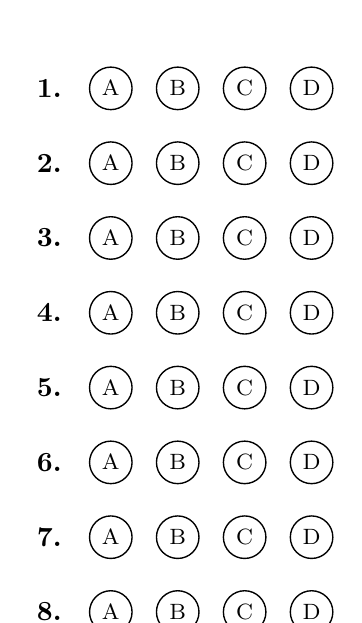
\begin{tikzpicture}[x=1cm,y=1cm]
\node[anchor=east] at (0.55,0.00) {\textbf{1.}};
\draw[line width=0.5pt] (1.05,0.00) circle (0.27);
\node at (1.05,0.00) {\footnotesize A};
\draw[line width=0.5pt] (1.90,0.00) circle (0.27);
\node at (1.90,0.00) {\footnotesize B};
\draw[line width=0.5pt] (2.75,0.00) circle (0.27);
\node at (2.75,0.00) {\footnotesize C};
\draw[line width=0.5pt] (3.60,0.00) circle (0.27);
\node at (3.60,0.00) {\footnotesize D};
\node[anchor=east] at (0.55,-0.95) {\textbf{2.}};
\draw[line width=0.5pt] (1.05,-0.95) circle (0.27);
\node at (1.05,-0.95) {\footnotesize A};
\draw[line width=0.5pt] (1.90,-0.95) circle (0.27);
\node at (1.90,-0.95) {\footnotesize B};
\draw[line width=0.5pt] (2.75,-0.95) circle (0.27);
\node at (2.75,-0.95) {\footnotesize C};
\draw[line width=0.5pt] (3.60,-0.95) circle (0.27);
\node at (3.60,-0.95) {\footnotesize D};
\node[anchor=east] at (0.55,-1.90) {\textbf{3.}};
\draw[line width=0.5pt] (1.05,-1.90) circle (0.27);
\node at (1.05,-1.90) {\footnotesize A};
\draw[line width=0.5pt] (1.90,-1.90) circle (0.27);
\node at (1.90,-1.90) {\footnotesize B};
\draw[line width=0.5pt] (2.75,-1.90) circle (0.27);
\node at (2.75,-1.90) {\footnotesize C};
\draw[line width=0.5pt] (3.60,-1.90) circle (0.27);
\node at (3.60,-1.90) {\footnotesize D};
\node[anchor=east] at (0.55,-2.85) {\textbf{4.}};
\draw[line width=0.5pt] (1.05,-2.85) circle (0.27);
\node at (1.05,-2.85) {\footnotesize A};
\draw[line width=0.5pt] (1.90,-2.85) circle (0.27);
\node at (1.90,-2.85) {\footnotesize B};
\draw[line width=0.5pt] (2.75,-2.85) circle (0.27);
\node at (2.75,-2.85) {\footnotesize C};
\draw[line width=0.5pt] (3.60,-2.85) circle (0.27);
\node at (3.60,-2.85) {\footnotesize D};
\node[anchor=east] at (0.55,-3.80) {\textbf{5.}};
\draw[line width=0.5pt] (1.05,-3.80) circle (0.27);
\node at (1.05,-3.80) {\footnotesize A};
\draw[line width=0.5pt] (1.90,-3.80) circle (0.27);
\node at (1.90,-3.80) {\footnotesize B};
\draw[line width=0.5pt] (2.75,-3.80) circle (0.27);
\node at (2.75,-3.80) {\footnotesize C};
\draw[line width=0.5pt] (3.60,-3.80) circle (0.27);
\node at (3.60,-3.80) {\footnotesize D};
\node[anchor=east] at (0.55,-4.75) {\textbf{6.}};
\draw[line width=0.5pt] (1.05,-4.75) circle (0.27);
\node at (1.05,-4.75) {\footnotesize A};
\draw[line width=0.5pt] (1.90,-4.75) circle (0.27);
\node at (1.90,-4.75) {\footnotesize B};
\draw[line width=0.5pt] (2.75,-4.75) circle (0.27);
\node at (2.75,-4.75) {\footnotesize C};
\draw[line width=0.5pt] (3.60,-4.75) circle (0.27);
\node at (3.60,-4.75) {\footnotesize D};
\node[anchor=east] at (0.55,-5.70) {\textbf{7.}};
\draw[line width=0.5pt] (1.05,-5.70) circle (0.27);
\node at (1.05,-5.70) {\footnotesize A};
\draw[line width=0.5pt] (1.90,-5.70) circle (0.27);
\node at (1.90,-5.70) {\footnotesize B};
\draw[line width=0.5pt] (2.75,-5.70) circle (0.27);
\node at (2.75,-5.70) {\footnotesize C};
\draw[line width=0.5pt] (3.60,-5.70) circle (0.27);
\node at (3.60,-5.70) {\footnotesize D};
\node[anchor=east] at (0.55,-6.65) {\textbf{8.}};
\draw[line width=0.5pt] (1.05,-6.65) circle (0.27);
\node at (1.05,-6.65) {\footnotesize A};
\draw[line width=0.5pt] (1.90,-6.65) circle (0.27);
\node at (1.90,-6.65) {\footnotesize B};
\draw[line width=0.5pt] (2.75,-6.65) circle (0.27);
\node at (2.75,-6.65) {\footnotesize C};
\draw[line width=0.5pt] (3.60,-6.65) circle (0.27);
\node at (3.60,-6.65) {\footnotesize D};
\end{tikzpicture}
\end{minipage}\hfill
\begin{minipage}[t]{0.32\textwidth}\centering
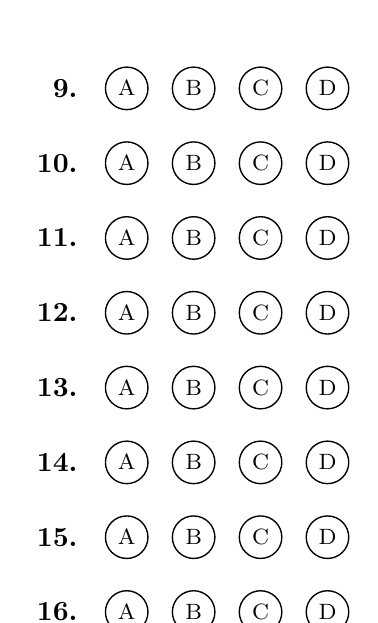
\begin{tikzpicture}[x=1cm,y=1cm]
\node[anchor=east] at (0.55,0.00) {\textbf{9.}};
\draw[line width=0.5pt] (1.05,0.00) circle (0.27);
\node at (1.05,0.00) {\footnotesize A};
\draw[line width=0.5pt] (1.90,0.00) circle (0.27);
\node at (1.90,0.00) {\footnotesize B};
\draw[line width=0.5pt] (2.75,0.00) circle (0.27);
\node at (2.75,0.00) {\footnotesize C};
\draw[line width=0.5pt] (3.60,0.00) circle (0.27);
\node at (3.60,0.00) {\footnotesize D};
\node[anchor=east] at (0.55,-0.95) {\textbf{10.}};
\draw[line width=0.5pt] (1.05,-0.95) circle (0.27);
\node at (1.05,-0.95) {\footnotesize A};
\draw[line width=0.5pt] (1.90,-0.95) circle (0.27);
\node at (1.90,-0.95) {\footnotesize B};
\draw[line width=0.5pt] (2.75,-0.95) circle (0.27);
\node at (2.75,-0.95) {\footnotesize C};
\draw[line width=0.5pt] (3.60,-0.95) circle (0.27);
\node at (3.60,-0.95) {\footnotesize D};
\node[anchor=east] at (0.55,-1.90) {\textbf{11.}};
\draw[line width=0.5pt] (1.05,-1.90) circle (0.27);
\node at (1.05,-1.90) {\footnotesize A};
\draw[line width=0.5pt] (1.90,-1.90) circle (0.27);
\node at (1.90,-1.90) {\footnotesize B};
\draw[line width=0.5pt] (2.75,-1.90) circle (0.27);
\node at (2.75,-1.90) {\footnotesize C};
\draw[line width=0.5pt] (3.60,-1.90) circle (0.27);
\node at (3.60,-1.90) {\footnotesize D};
\node[anchor=east] at (0.55,-2.85) {\textbf{12.}};
\draw[line width=0.5pt] (1.05,-2.85) circle (0.27);
\node at (1.05,-2.85) {\footnotesize A};
\draw[line width=0.5pt] (1.90,-2.85) circle (0.27);
\node at (1.90,-2.85) {\footnotesize B};
\draw[line width=0.5pt] (2.75,-2.85) circle (0.27);
\node at (2.75,-2.85) {\footnotesize C};
\draw[line width=0.5pt] (3.60,-2.85) circle (0.27);
\node at (3.60,-2.85) {\footnotesize D};
\node[anchor=east] at (0.55,-3.80) {\textbf{13.}};
\draw[line width=0.5pt] (1.05,-3.80) circle (0.27);
\node at (1.05,-3.80) {\footnotesize A};
\draw[line width=0.5pt] (1.90,-3.80) circle (0.27);
\node at (1.90,-3.80) {\footnotesize B};
\draw[line width=0.5pt] (2.75,-3.80) circle (0.27);
\node at (2.75,-3.80) {\footnotesize C};
\draw[line width=0.5pt] (3.60,-3.80) circle (0.27);
\node at (3.60,-3.80) {\footnotesize D};
\node[anchor=east] at (0.55,-4.75) {\textbf{14.}};
\draw[line width=0.5pt] (1.05,-4.75) circle (0.27);
\node at (1.05,-4.75) {\footnotesize A};
\draw[line width=0.5pt] (1.90,-4.75) circle (0.27);
\node at (1.90,-4.75) {\footnotesize B};
\draw[line width=0.5pt] (2.75,-4.75) circle (0.27);
\node at (2.75,-4.75) {\footnotesize C};
\draw[line width=0.5pt] (3.60,-4.75) circle (0.27);
\node at (3.60,-4.75) {\footnotesize D};
\node[anchor=east] at (0.55,-5.70) {\textbf{15.}};
\draw[line width=0.5pt] (1.05,-5.70) circle (0.27);
\node at (1.05,-5.70) {\footnotesize A};
\draw[line width=0.5pt] (1.90,-5.70) circle (0.27);
\node at (1.90,-5.70) {\footnotesize B};
\draw[line width=0.5pt] (2.75,-5.70) circle (0.27);
\node at (2.75,-5.70) {\footnotesize C};
\draw[line width=0.5pt] (3.60,-5.70) circle (0.27);
\node at (3.60,-5.70) {\footnotesize D};
\node[anchor=east] at (0.55,-6.65) {\textbf{16.}};
\draw[line width=0.5pt] (1.05,-6.65) circle (0.27);
\node at (1.05,-6.65) {\footnotesize A};
\draw[line width=0.5pt] (1.90,-6.65) circle (0.27);
\node at (1.90,-6.65) {\footnotesize B};
\draw[line width=0.5pt] (2.75,-6.65) circle (0.27);
\node at (2.75,-6.65) {\footnotesize C};
\draw[line width=0.5pt] (3.60,-6.65) circle (0.27);
\node at (3.60,-6.65) {\footnotesize D};
\end{tikzpicture}
\end{minipage}\hfill
\begin{minipage}[t]{0.32\textwidth}\centering
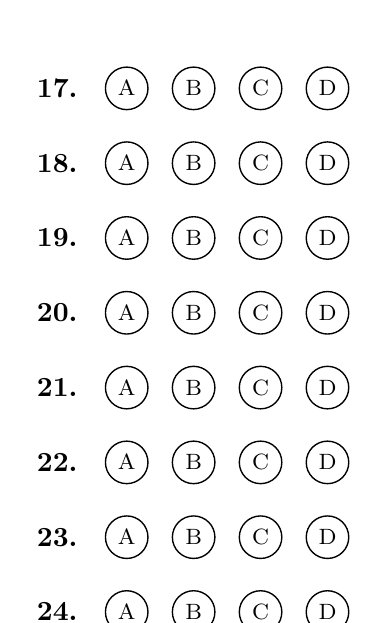
\begin{tikzpicture}[x=1cm,y=1cm]
\node[anchor=east] at (0.55,0.00) {\textbf{17.}};
\draw[line width=0.5pt] (1.05,0.00) circle (0.27);
\node at (1.05,0.00) {\footnotesize A};
\draw[line width=0.5pt] (1.90,0.00) circle (0.27);
\node at (1.90,0.00) {\footnotesize B};
\draw[line width=0.5pt] (2.75,0.00) circle (0.27);
\node at (2.75,0.00) {\footnotesize C};
\draw[line width=0.5pt] (3.60,0.00) circle (0.27);
\node at (3.60,0.00) {\footnotesize D};
\node[anchor=east] at (0.55,-0.95) {\textbf{18.}};
\draw[line width=0.5pt] (1.05,-0.95) circle (0.27);
\node at (1.05,-0.95) {\footnotesize A};
\draw[line width=0.5pt] (1.90,-0.95) circle (0.27);
\node at (1.90,-0.95) {\footnotesize B};
\draw[line width=0.5pt] (2.75,-0.95) circle (0.27);
\node at (2.75,-0.95) {\footnotesize C};
\draw[line width=0.5pt] (3.60,-0.95) circle (0.27);
\node at (3.60,-0.95) {\footnotesize D};
\node[anchor=east] at (0.55,-1.90) {\textbf{19.}};
\draw[line width=0.5pt] (1.05,-1.90) circle (0.27);
\node at (1.05,-1.90) {\footnotesize A};
\draw[line width=0.5pt] (1.90,-1.90) circle (0.27);
\node at (1.90,-1.90) {\footnotesize B};
\draw[line width=0.5pt] (2.75,-1.90) circle (0.27);
\node at (2.75,-1.90) {\footnotesize C};
\draw[line width=0.5pt] (3.60,-1.90) circle (0.27);
\node at (3.60,-1.90) {\footnotesize D};
\node[anchor=east] at (0.55,-2.85) {\textbf{20.}};
\draw[line width=0.5pt] (1.05,-2.85) circle (0.27);
\node at (1.05,-2.85) {\footnotesize A};
\draw[line width=0.5pt] (1.90,-2.85) circle (0.27);
\node at (1.90,-2.85) {\footnotesize B};
\draw[line width=0.5pt] (2.75,-2.85) circle (0.27);
\node at (2.75,-2.85) {\footnotesize C};
\draw[line width=0.5pt] (3.60,-2.85) circle (0.27);
\node at (3.60,-2.85) {\footnotesize D};
\node[anchor=east] at (0.55,-3.80) {\textbf{21.}};
\draw[line width=0.5pt] (1.05,-3.80) circle (0.27);
\node at (1.05,-3.80) {\footnotesize A};
\draw[line width=0.5pt] (1.90,-3.80) circle (0.27);
\node at (1.90,-3.80) {\footnotesize B};
\draw[line width=0.5pt] (2.75,-3.80) circle (0.27);
\node at (2.75,-3.80) {\footnotesize C};
\draw[line width=0.5pt] (3.60,-3.80) circle (0.27);
\node at (3.60,-3.80) {\footnotesize D};
\node[anchor=east] at (0.55,-4.75) {\textbf{22.}};
\draw[line width=0.5pt] (1.05,-4.75) circle (0.27);
\node at (1.05,-4.75) {\footnotesize A};
\draw[line width=0.5pt] (1.90,-4.75) circle (0.27);
\node at (1.90,-4.75) {\footnotesize B};
\draw[line width=0.5pt] (2.75,-4.75) circle (0.27);
\node at (2.75,-4.75) {\footnotesize C};
\draw[line width=0.5pt] (3.60,-4.75) circle (0.27);
\node at (3.60,-4.75) {\footnotesize D};
\node[anchor=east] at (0.55,-5.70) {\textbf{23.}};
\draw[line width=0.5pt] (1.05,-5.70) circle (0.27);
\node at (1.05,-5.70) {\footnotesize A};
\draw[line width=0.5pt] (1.90,-5.70) circle (0.27);
\node at (1.90,-5.70) {\footnotesize B};
\draw[line width=0.5pt] (2.75,-5.70) circle (0.27);
\node at (2.75,-5.70) {\footnotesize C};
\draw[line width=0.5pt] (3.60,-5.70) circle (0.27);
\node at (3.60,-5.70) {\footnotesize D};
\node[anchor=east] at (0.55,-6.65) {\textbf{24.}};
\draw[line width=0.5pt] (1.05,-6.65) circle (0.27);
\node at (1.05,-6.65) {\footnotesize A};
\draw[line width=0.5pt] (1.90,-6.65) circle (0.27);
\node at (1.90,-6.65) {\footnotesize B};
\draw[line width=0.5pt] (2.75,-6.65) circle (0.27);
\node at (2.75,-6.65) {\footnotesize C};
\draw[line width=0.5pt] (3.60,-6.65) circle (0.27);
\node at (3.60,-6.65) {\footnotesize D};
\end{tikzpicture}
\end{minipage}\hfill

\vspace{3em}
\begin{center}
\large Score \quad \underline{\hspace{2cm}} \,/\, 24
\end{center}


\newpage
\begin{center}
  {\Large\bfseries Formula Sheet}\\[3pt]
  {\small\itshape Use this page only if your exam provides a formula sheet.}\\[2pt]
  \rule{\textwidth}{0.4pt}
\end{center}

\subsection*{Fitness}
\begin{center}\renewcommand{\arraystretch}{2.1}
\begin{tabular}{r@{\;}l@{\qquad}l}
  \(w\) & \(=\ \text{viability} \times \text{fecundity}\) & absolute fitness, offspring left per zygote\\
  \(W\) & \(=\ w / w_{\max}\) & relative fitness\\
  \(s\) & \(=\ 1 - W\) & selection coefficient
\end{tabular}\end{center}

\subsection*{Mean fitness and the general equation}
\begin{align*}
  \overline{W} &= f(AA)\,W_{AA} + f(Aa)\,W_{Aa} + f(aa)\,W_{aa}\\[4pt]
  q' &= \frac{\tfrac{1}{2}\,f(Aa)\,W_{Aa} + f(aa)\,W_{aa}}{\overline{W}}, \qquad \Delta q = q' - q
\end{align*}
Under Hardy--Weinberg, \(f(AA)=p^2\), \(f(Aa)=2pq\), \(f(aa)=q^2\). With counted individuals that selection acts on directly, use the counted frequencies.

\subsection*{Average excess}
\begin{align*}
  \alpha_a &= q\,W_{aa} + p\,W_{Aa} - \overline{W}, & \Delta q &= \frac{q}{\overline{W}}\,\alpha_a\\[4pt]
  \alpha_A &= p\,W_{AA} + q\,W_{Aa} - \overline{W}, & \Delta p &= \frac{p}{\overline{W}}\,\alpha_A
\end{align*}
Requires Hardy--Weinberg genotype frequencies.

\subsection*{Special models (\(q\) is always the allele selected against)}
\begin{align*}
  \text{Against the recessive:}\quad \Delta q &= \frac{-s\,p\,q^2}{1 - s\,q^2}\\[4pt]
  \text{Against the dominant:}\quad \Delta q &= \frac{-s\,p^2 q}{1 - 2sq + sq^2}
\end{align*}

\subsection*{Heterozygote advantage or disadvantage}
\[
  \hat{q} = \frac{s_1}{s_1 + s_2}
\]
with \(s_1\) for the \(p\) homozygote and \(s_2\) for the \(q\) homozygote. The equilibrium is stable under heterozygote advantage and unstable under heterozygote disadvantage.

\label{LastPage}
\end{document}